\documentclass[12pt, titlepage, oneside]{article}

\usepackage[margin=1in]{geometry}
\usepackage{siunitx, booktabs, amsmath, enumitem, pdfpages,mathrsfs,tabularx,caption, graphicx, pgfplots, textcomp,wrapfig, commath, svg, amsfonts, relsize}
\usepackage{parskip}
\usepackage[siunitx]{circuitikz}
\sisetup{detect-weight=true, detect-family=true}
\renewcommand{\vec}[1]{\oldvec{\bm{#1}}}
\renewcommand{\hat}[1]{\oldhat{\bm{#1}}}
\renewcommand{\b}[1]{\textbf{#1}}
\newcommand{\de}[1]{\noindent\fbox{\parbox{\textwidth}{#1}}}



\newcommand{\items}{\begin{itemize}}
\newcommand{\eitems}{\end{itemize}}


\newcommand{\ex}{Ex. }
\newcommand{\exe}{_}

\newcommand{\n}{\cap}
\renewcommand{\u}{\cup}


\begin{document}
	
	\textbf{ELECENG 3TQ3}\\
	\textbf{Elston A.}
	
\section{Lecture 5}

\subsection{Bernoulli Trials}

From the last example in Lecture 4, we talked about repeated trails with a coin toss. 

Consider tossing a coin 5 times, recording the outcomes, and repeating the whole process 10 times. We can say that one outcome would lead to heads and the other outcome would lead to tails. This is in a way a "success" and "failure" type experiment. We would like to know how to deal with such an event.

Lets continue to a probably more cooler scenario. Consider Intel's manufacturing process in which 100 CPUs are selected for testing.
Assume that the probability of a CPU manufactured at that location failing the test is 0.02. What is the probability that of the 100 CPUs tested that k will pass the test.

The answer is simply
\begin{align}
{100\choose n} (0.98)^n (0.02)^{100-n}
\end{align}
Since we do not care about which order the CPUs failed or passed, we need to only consider the combination rather than the permutation. We know that $(0.98)^n(0.02)^{100-n}$ is the probability that if you picked a single CPU if it would pass, but since we are picking 100 CPUs we need to multiply by the total combination to see the actual pass rate. 

\subsection{Sub Experiment}

Instead of two outcomes, we may have multiple outcomes for every trial shown as $s_1,s_2,\dots,s_m$. We denote the probability of outcome $s_i$ as $p_i$. If we have $n$ trials, then the sum of all the $m$ outcomes during an experiment $n_1 + n_2 + \dots + n_m = n$. The probability of the outcome is given as
\begin{align}
{n \choose n_1,n_2,\dots,n_m} p_1^{n_1} p_2^{n_2} \dots p_m^{n_m}
\end{align}
The coefficient in the bracket is called the multinomial coefficient and represent permutation with repetition. This is because we can have multiple outcomes being the same.

\b{note}: The multinomial coefficient is calculated as follows
\begin{align}
{n \choose n_1, n_2, \dots, n_m} = \frac{n!}{n_1! n_2! \dots n_m!}
\end{align}

\ex Let us consider the set $\{a,a,b,b\}$. To final all the distinct permutations of this set, we can see it is as follows:
${aabb,abab,abba,baab,baba,bbaa}$ so the answer is $6$ NOT $4!=24$. To find the distinct permutations, we need to divide the number of permutations that are considered as repetitions
\begin{align}
{4! \choose 2,2} = \frac{4!}{2!2!} = 6
\end{align}
\ex How many 7 digit numbers can you create using $0,0,0,0,1,2,3$ if we ignore numbers that begin with zero
\begin{align}
{7 \choose 4} = 7!/4! = 210 
\end{align}

\subsection{Reliability}
Deals with the problem in which we want to find the probability that a particular system consisting of multiple components is all working properly.

The two main types to consider are series and parallel systems. Series systems needs every component to work whereas parallel needs at least one component to work.

We \b{ALWAYS} consider the probabilities to be independent unless specified otherwise

\ex
\begin{figure}[h]
	\centering
	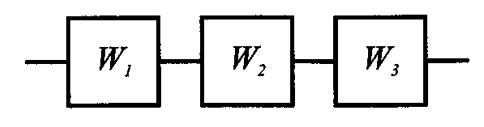
\includegraphics[width=0.7\linewidth]{../Lecture4/images/series}
	\caption{Series systems}
	\label{fig:series}
\end{figure}

Given the probability of each component $W_i$ working is $P(W_i)$. 

In this case we see the probability of the system working would be 
\begin{align}
P[W_1W_2W_3] = P[W_1]P[W_2]P[W_3]
\end{align}
The probability of failure would be
\begin{align}
P[W_1 \u W_2 \u W_3] = 1-P[W_1]P[W_2]P[W_3]
\end{align}
We can see this is a direct result from our talks about independent in the previous lecture.

\ex
\begin{figure}[h]
	\centering
	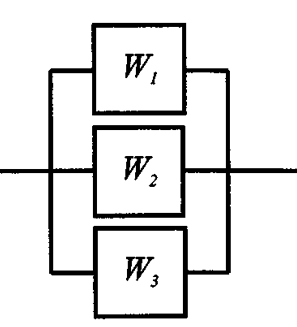
\includegraphics[width=0.4\linewidth]{../Lecture4/images/parallel}
	\caption{Parallel systems}
	\label{fig:parallel}
\end{figure}

With the same notation as the previous example, we can see the probability of this system working is given as follows:
\begin{align}
&P[W_1 \u W2 \u W3] = P[W_1] + P[W_2 \u W_3] - P[W_1 \n (W_2 \u W_3)]\\
&= P[W_1] + P[W_2] + P[W_3] - P[W_1\u W_2] - P[W_1 \u W_3] - P[W_2 \u W_3] + P[W_1 \u W_2 \u W_3]
\end{align}
This way is also too tedious and wastes too much time. Since we know the events are independent, we can use the following to get the same result
\begin{align}
P[W_1 \u W_2 \u W_3] = 1- P[W_1 W_2 W_3] = 1-P[W_1]P[W_2]P[W_3]
\end{align}
\end{document}
